In this chapter we will make an overview about the aspects of Neural Random-Access Machines \cite{NRAM:2016}, a model inspired by the Random Access Machine (not to confuse with Random Access Memory) and ANN-based that has as scope the learning of algorithms. So starting from a simplified design that does not include an external memory to the version with this latter. Then we will introduce the design that we have adopted for the modules which is not included in the original paper.


\section{Registers only model}
The simplified NRAM model can be divided in three main pieces: the controller, the registers and the gates (modules). The central part is the controller that can be a FNN or an LSTM and is the only part that is trainable. The registers is a set of variable-sized memory cells. The point of contact between controller and the registers is a set of gates (named also modules) with which the controller, connecting these latter as a "logic" or "fuzzy" circuit, can modify the registers value. 

\subsubsection*{The registers}
At high level, the registers contain integer values, but with the objective of using the gradient descent the registers does not contain directly the integer values but the fuzzy version of them, so the NRAM can be thus fully differentiable. In other word, let $N\ =\ \{0,\ 1,\ 2,\ \dots,\ I - 1\}$ a set of integers associated to the NRAM for some integer constant $I$, then each register contains a vector $p \in \textrm{I\!R}^{|N|}$ where to every cell is associated an integer value of the set M. So then every cell of the vector contains the probability that the associated register contain the integer value associated to the cell. Furthermore the vector values must satisfy $p_{i} \geq 0$ and $\sum\limits_{i = 0}^{|N|} p_{i} = 1$.

\subsubsection*{The modules}
In the original paper three types of gates have been introduced: constant, unary and binary. Let $M\ =\ \{m_1, m_2, \dots, m_Q \}$ the set of the modules, then each of them can be represented as a function as follow
\begin{center}
	\begin{equation}
		\begin{split}		
			m_i \in N & \textrm{ (Constant modules)} \\
			m_i: N \rightarrow N & \textrm{ (Unary modules)} \\
			m_i: N \times N \rightarrow N & \textrm{ (Binary modules)}
		\end{split}
	\end{equation}
\end{center}
In the paper is used always the same sequence of fourteen modules: Read (described in the section \ref{sec:nram-memory}), Zero(a, b) = 0, One(a, b) = 1, Two(a, b) = 2, Inc(a, b) = (a + 1) mod I, Add(a, b) = (a + b) mod I, Sub(a, b) = (a - b) mod I, Dec(a, b) = (a - 1) mod I, Less-Than(a, b) = [a $\le$ b], Less-Or-Equal-Than(a, b) = [a $\leq$ b], Equal-Than(a, b) = [a = b], Min($a$, $b$) = $\min(a, b)$, Max($a$, $b$) = $\max(a, b)$, Write( (described in the section \ref{sec:nram-memory}). Using always the same sequence is important, because a different permutation of the set M can bring the machine to not converge. Furthermore for the same reason of the registers they have to work over probability distribution, so the \textbf{a} and \textbf{b} are vector and not single integer values.

%Since the original paper does not give any further information about the modules except for the Read and the Write, we have implemented them in the fuzzy version (the integer version is as above) as follows. So let two vectors \textbf{a} and \textbf{b} of possibility distribution over N we have 
%\begin{itemize}
%	\item[$1.$] \textbf{Inc(a, b)} Given the vector \textbf{a} the incremented vector corresponds to a right shift of \textbf{a}, this because the possibility of a particular integer value $i$ in the output is the old possibility value of $i-1$ in the initial vector.
%	\item[$2.$]{\textbf{Add(a, b)} Given the vectors \textbf{a} and \textbf{b}, the output of gate Add corresponds to a new vector where each element $o_i$ contains the summation of joint possibility of all the cases in which the elements of the set $N$ produce the associated $i$ to $o_i$ through summation. For example given $a = [0.2, 0.7, 0.1]$ and $b = [0.3, 0.5, 0.2]$ the output is $Add(a, b) = [0.25, 0.33, 0.42]$}
%	\item[$3.$] \textbf{Sub(a, b)} As the gate Add, but considering the subtraction instead the summation.
%	\item[$4.$] \textbf{Dec(a, b)} As the gate Inc, but with a left shift.
%	\item[$5.$] \textbf{Less-Than(a, b)} Given the vectors \textbf{a} and \textbf{b}, the output is a vector where in the position $1^{st}$ contains the summation of joint possibility of all the cases in which the indexes of the vector \textbf{a}, called $x$, are smaller respect the indexes of \textbf{b}, called $y$, and in the index $0^{th}$ the joint possibility of all the remaining cases.
%	\item[$5.$] \textbf{Less-Or-Equal-Than(a, b)} Similar to Less-Than, but considering also the equality of the indexes.
%	\item[$6.$] \textbf{Equality-Test(a, b)} Similar to Less-Than, but considering only the equality of the indexes.
%	\item[$7.$] \textbf{Min(a, b)} Given the vectors \textbf{a} and \textbf{b}, returns the smaller vector, i.e. the vector that has the greatest value in the $1^{st}$ index of the output vector of Less-Than.
%	\item[$7.$] \textbf{Max(a, b)} Given the vectors \textbf{a} and \textbf{b}, returns the smaller vector, i.e. the vector that has the greatest value in the $0^{th}$ index of the output vector of Less-Than.
%\end{itemize}

\begin{figure}[t!]
	\centering
	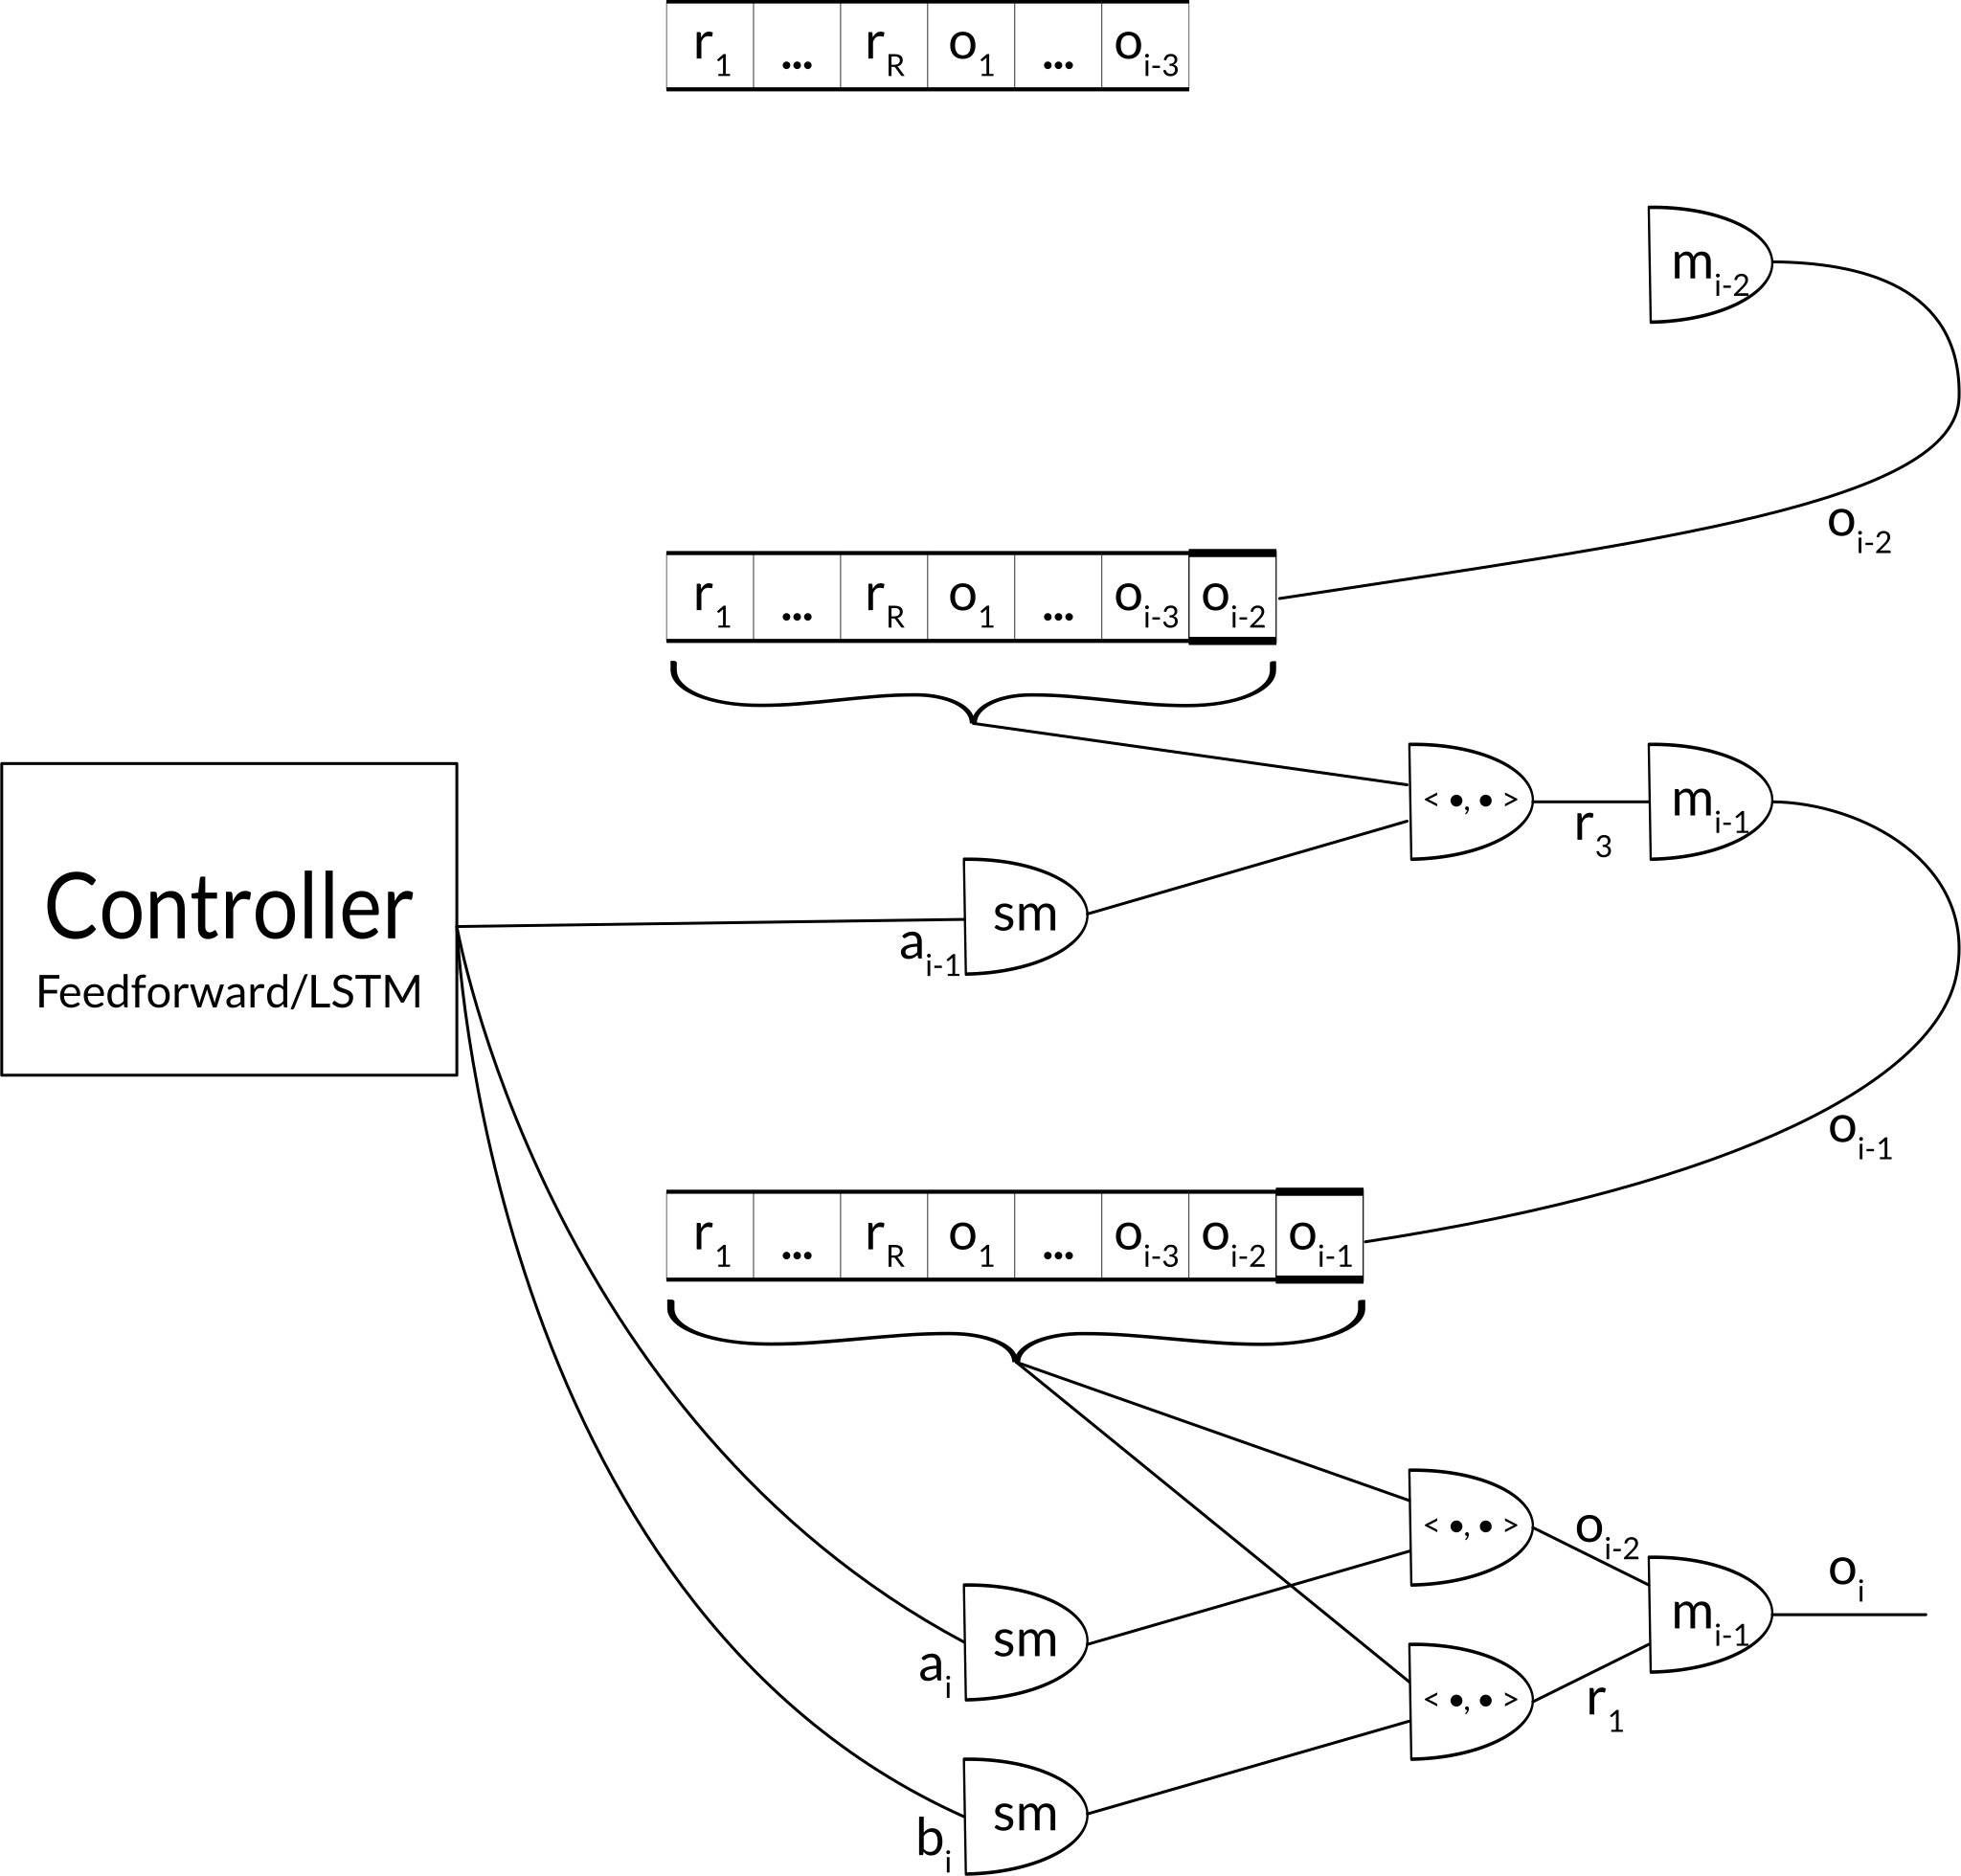
\includegraphics[width=\textwidth]{figures/register-only-model.png}
	\caption{Extract of execution of NRAM circuit. The node with \textbf{sm} refers to a softmax activation function and the $<\cdot$, $\cdot>$ to a weighted average (in this case between the registers plus previous modules output respect to the coefficient \textbf{softmax}($\dots$)). With the weighted average the NRAM selects one input, obviously indicated by the coefficient, with which the next module is fed.}
	\label{fig:register-only-model}
\end{figure}

\subsection{Execution flow of register-only model}\label{subsec:execution-register-only}
For a better comprehension of the NRAM execution can be read the pseudocode in the algorithm \ref{alg:nram}.
\begin{algorithm}
	\begin{algorithmic}[1]
		\State{Let a controller (FFN or LSTM)}
		\State{Let $R$ register}
		\State{Let $M$ a set of modules}
		\State{Let $T$ timesteps}
		\For{each timestep $t \in T$}\label{lst:nram:line-5}
			\State Controller gets as inputs the registers content\label{lst:nram:line-6}
			\If{controller is a LSTM}
				\State Controller update its internal state
			\EndIf
			\State Controller outputs one-shot the configuration of the NRAM 
			\label{lst:nram:line-8}
			\State The "fuzzy circuit" is executed \label{lst:nram:line-9}
			\State The values of the registers is updated\label{lst:nram:line-10}
		\EndFor
	\end{algorithmic}
	\caption{Execution of the NRAM without the memory}\label{alg:nram}
\end{algorithm}

The execution of the NRAM starts at the line \ref{lst:nram:line-5} and continue for all the timesteps. At the line \ref{lst:nram:line-8}, after the controller gets the input from the registers, this latter is executed generating a new configuration that is used at the lines \ref{lst:nram:line-9} and \ref{lst:nram:line-10}. 
This latter indicates how the circuit is structured, i.e. indicates for each gate the input source, that could be a register or the output of another gate.

In other words, the inputs for a gates $m_i$ is chosen by the controller from the set $\{r_{1}, \dots, r_{R}, o_{1}, \dots, o_{i-1}\}$ where:
\begin{itemize}
	\item $r_j$ is the content of the $j^{th}$ register
	\item $o_j$ is the content of the output of the $j^{th}$ previous gate respect to the current $m_i$
\end{itemize}
selected through a weighted average with a coefficient as follow
\begin{center}
	\begin{equation}
		(r_1, r_2, \dots, r_R, o_1, o_2, \dots, o_{i-1})^T\textbf{softmax}(s_i)
	\end{equation}
\end{center}
where $\textrm{s}_i \in \textrm{I\!R}^{R+i-1}$ is a generic vector that represents the input source for the $i^{th}$ gate and the $\textbf{softmax}(s_i)$ is called coefficient. \newline
So let $m_i \in M$ the $i^{th}$ module in $M$, $m_i$ is executed as follows
\begin{itemize}
	\item{Constant gate
		\begin{equation}
			o_i = m_i()
		\end{equation}
	}
	\item{Unary gate
		\begin{equation}
			o_i = m_i((r_1, \dots, r_R, o_1, \dots, o_{i-1})^T\textbf{softmax}(a_i))
		\end{equation}
	}
	\item{Binary gate
		\begin{equation}
			o_i = m_i((r_1, \dots, r_R, o_1, \dots, o_{i-1})^T\textbf{softmax}(a_i), (r_1, \dots, r_R, o_1, \dots, o_{i-1})^T\textbf{softmax}(b_i))
		\end{equation}
	}
\end{itemize}
where, as stated previously, $a_i, b_i \in \textrm{I\!R}^{R+i-1}$ are produced by the controller and the $o_i$ is the output that is appended to the set $\{r_{1}, \dots, r_{R}, o_{1}, \dots, o_{i-1}\}$ and used later for the subsequent modules.

Since the registers $r_j$ contain probability distributions, the inputs of the modules are also probability distributions because are weighted averages of probability distributions. Hence, in this way, the gates are extended to work over probability distributions and because the inputs of these latter are probability distributions also the output is a probability distribution as follows:
\begin{center}
	\begin{equation}
		\mathop{\forall}\limits_{c \in N} P(m_i(A, B) = c) = \sum\limits_{a,b \in N} P(A = a)P(B = b)[m_i(a, b) = c]
	\end{equation}
\end{center}

At the same time of the emission of the vectors $a_{i}, b_{i} \in \textrm{I\!R}^{R+i-1}$ are also emitted the vectors $c_i \in \textrm{I\!R}^{R+|M|}$ for $i = 1, 2, \dots, R$, which indicate the sources, that can be the register content at timestep $t-1$ or a module output at the current timestep $t$, from which the new registers content is get. So after the circuit is executed, at the line \ref{lst:nram:line-10}, the registers content is updated as follows:
\begin{center}
	\begin{equation}
		\begin{split}
			r_i^{(t + 1)} = (r_1^{(t)}, \dots, r_R^{(t)}, o_1, \dots, o_{|M|})^T\textbf{softmax}(c_i) &,\ \ \ i = 1,\dots,R
		\end{split}
	\end{equation}
\end{center}

As stated previously, at the line \ref{lst:nram:line-6} the controller get some input from the registers. This input could be all the registers content, but in this way the controller's parameters would depend directly on M. This case is undesirable because this latter could learn the specific problem on which it trains, preventing this latter to generalize to different size of M. 

\begin{wrapfigure}{r}{0.5\textwidth}
	\centering
	\includegraphics[width=0.5\textwidth]{figures/circuit.png}
	\caption{Example of NRAM circuit. With the circles are represented the registers and with the rectangles are represented the various circuits. The registers with the apex are those that are modified in the timestep. The labels x and y represent the values order for the gates (obviously if it is violated, a gate produces a different result). The modules Read and Write are presented in the next section.}
	\label{fig:example-circuit}
\end{wrapfigure}

Hence to resolve this inconvenient, in the original paper the controller receives from all the registers $R$ only $P(r_{i} = 0)$, i.e. the probability that a register content is equal to zero. Another possibility that we have experimented is to give as input to the controller the integer with the greatest probability for each register $r_{i}$. In other words what we have done is to convert the probability distribution contained in the registers into integer, using these as input of the controller. We have tested and compared this last solution with the original, all the results can be read in the chapter \ref{experiments}

Both the solutions limits the information available to the controller, forcing it to solve the problem with the modules instead to its own, and reduces the problem complexity.

\section{Memory augmented model}\label{sec:nram-memory}
The previously described model work only with the registers. Hence to make the ANN learn an algorithm, the learning process starts initializing the registers with the problem starting input sequence. The main disadvantage of this solution is that the model is constrained to the number of the registers, unable to generalize to longer sequence of a problem because, simply, the model cannot process sequences longer than the number of the registers which is constant.

Hence to resolve this problem, the model is augmented with a variable-sized memory tape of $|N|$ memory cells, where each of them stores a distribution over the set $N$. Each distribution both in registers and in memory could be seen as a fuzzy address and so used by the NRAM as a fuzzy pointer to a memory location. The memory can be formalized as a matrix $\mathcal{M} \in \textrm{I\!R}_{|N|}^{|N|}$, where a value $\mathcal{M}_{i,j}$ is the probability that the $i^{th}$ memory cell contains the $j^{th}$ integer value.

Hence, to interact with the memory the NRAM contains another two modules:
\begin{itemize}
	\item{\textbf{Read}: this module takes as input a pointer and returns as output the memory content at the location indicated by the pointer. This behaviour is the same both the pointer is an integer or a probability distribution, what change is the system with which the module access the memory cell. More precisely, if the pointer $p\in\textrm{I\!R}^{|N|}$ is a probability distribution represented as a column vector, then the module returns $\mathcal{M}^{T}p$.}
	\item{\textbf{Write}: this module takes as input a pointer and a value and returns zero. As for the \textbf{Read} module,  what change is the behaviour of the module due to the input type. In the case the inputs are probability distributions the module behave as follows:
\begin{center}
	\begin{equation}
	\mathcal{M} = (J - p)J^{T} \cdot \mathcal{M} + pa^{T}
	\end{equation}
\end{center}	
where $J \in \{1\}^{|N|}$ is a column vector and $\cdot$ denotes a coordinate-wise multiplication.}
\end{itemize}
The architecture of the memory augmented NRAM is presented in the figure \ref{fig:memory-nram}.

Recalling the learning process of the registers only model, in this case the memory is initialized with the problem starting input sequence used as a I/O device. In this way the controller can learn an algorithm operations over a sequence of limited size and later could apply them to a longer sequence.

\begin{figure}[t!]
	\centering
	\includegraphics[width=\textwidth]{figures/memory-augmented-model.png}
	\caption{Execution of the NRAM memory augmented architecture with $R$ = 4 registers. As can be seen the controllers get a registers \qq{binarized} version, with which coefficients and the $f_{i}$ are produced. As stated previously in subsection \ref{subsec:execution-register-only}, the coefficients are used to select connections that here are represented with solid lines. Instead, with the dashed connections are represented the interactions by the \textbf{Read} and \textbf{Write} modules with the memory.}
	\label{fig:perceptron-boundaries}
\end{figure}

Moreover, the NRAM use a system with which can decide if the execution can be terminated. Recalling that the execution is divided $T$ timesteps, in each of them the controller emits along the various $a, b, c$ vectors a scalar $f_{t} \in [0, 1]$\footnote{The controller emits a scalar $x_{i}$, with which is produced the $f_i = \textbf{sigmoid}(x_{i})$.}, defined in other words as the willingness of finish the execution in the current timestep $t$. Thus, starting from this we have that the probability that the execution is not finished in the previous timestep is $\prod\limits_{i=1}^{t-1}(1 - f_{i})$ and the probability that the output is produced in the current timestep is $p_{t} = f_{t} \cdot \prod\limits_{i=1}^{t-1}(1 - f_{i})$. 

As stated previously, the execution is continued for a maximum of timestep $T$, except for the previous cases, where the NRAM is forced to emits an output and, due to this, the probability to terminate is $p_{T} = 1 - \sum\limits_{i=1}^{T-1}p_{i}$ regardless of the $f_{T}$ of the last timestep.

\subsection{Cost function}
The NRAM is a more complex system respect to an ANN and due to this the cost function is not standard because it can not capture how much the neural network departs from the expected output because, simply, we do not have it. 

So let $\mathcal{M}^{(t)} \in \textrm{I\!R}^{|N|}_{|N|}$ the memory matrix at the end of the execution of the timestep $t$ and $(x, y) \in N^{|N|}$ a couple which contains the starting input sequence and the expected output sequence, the cost function is defined, only for the memory augmented version, as the expected negative log-likelihood of producing the correct output, i.e.
\begin{center}
	\begin{equation}
		-\sum\limits_{i=1}^{T}\Bigg(p_{t}\cdot\sum\limits_{i=1}^{|N|}log\Big(\mathcal{M}_{i, y_{i}}^{(t)}\Big)\Bigg)
	\end{equation}
\end{center}
where $y_i$ is the expected integer value at the $i^{th}$ memory cell, that here acts also as a pointer. The cost calculation is made only over the part of memory that contains the output leaving out the other parts. These latter are made available as a free memory that supports the NRAM execution.